\documentclass{standalone}
\usepackage{fontspec}
\usepackage{sourcecodepro}
\usepackage{tikz}
\usepackage{unicode-math}

\setmainfont{TeX Gyre Heros}
\setmonofont{Source Code Pro}
\setmathfont{TeX Gyre Schola Math}


\usetikzlibrary{matrix, positioning, decorations.pathreplacing, calligraphy, calc}

\tikzset{
  layout/.style={
    matrix of nodes,
    row sep=-\pgflinewidth,
    %column sep=-\pgflinewidth,
    column sep=2pt,
    nodes={rectangle, align=center, font=\ttfamily, text depth=0.25ex, text height=1em},
    minimum height=1.5em,
    text depth=0.5ex,
    text height=2ex,
    nodes in empty cells,
  },
  cls/.style={rectangle, align=center, font=\ttfamily, text depth=0.25ex, text height=1em},
  arr/.style={
    text width=10em
  },
  slegend/.style={
    decorate, decoration={calligraphic brace, amplitude=3pt, mirror}, line width=0.5pt,
    % node options
    align=center, midway, below, font=\ttfamily
  },
  legend/.style={
    decorate, decoration={calligraphic brace, amplitude=5pt, mirror}, line width=0.5pt,
    % node options
    align=center, midway, below, font=\ttfamily, text depth=0.25ex, text height=1em
  }
}

\begin{document}
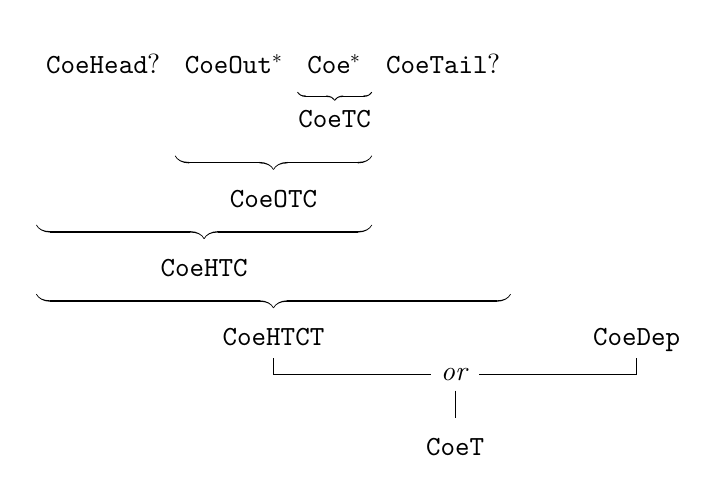
\begin{tikzpicture}
  \matrix (string) [layout] { %
    \node[](string-1-1){CoeHead$?$}; & \node[](string-1-2){CoeOut$^*$}; & \node[](string-1-3){Coe$^*$}; & \node[](string-1-4){CoeTail$?$};&\\%
  };
  \draw[slegend] ([yshift=-2pt]string-1-3.south west) -- ([yshift=-2pt]string-1-3.south east) node (coetc) [midway, below, yshift=-0.3em] {CoeTC};
  \draw[legend] ([yshift=-2.5em]string-1-2.south west) -- ([yshift=-2.5em]string-1-3.south east) node (coeotc) [midway, below, yshift=-0.5em] {CoeOTC};
  \draw[legend] ([yshift=-5em]string-1-1.south west) -- ([yshift=-5em]string-1-3.south east) node (coehtc) [midway, below, yshift=-0.5em] {CoeHTC};
  \draw[legend] ([yshift=-7.5em]string-1-1.south west) -- ([yshift=-7.5em]string-1-4.south east) node (coehtct) [midway, below, yshift=-0.5em] {CoeHTCT};
  \node[cls, right=9em of coehtct](coedep){CoeDep};
  \node(or) at ([yshift=-1.5em] $(coehtct)!0.5!(coedep)$){\textit{or}};
  \draw (coehtct.south) |- (or.west);
  \draw (coedep.south) |- (or.east);
  \node[cls, below=1em of or](coet){CoeT};
  \draw (or.south) -- (coet.north);
\end{tikzpicture}
\end{document}

% Local Variables:
% TeX-engine: luatex
% End:
